\let\negmedspace\undefined
\let\negthickspace\undefined
\documentclass[journal]{IEEEtran}
\usepackage[a5paper, margin=10mm, onecolumn]{geometry}
%\usepackage{lmodern} % Ensure lmodern is loaded for pdflatex
\usepackage{tfrupee} % Include tfrupee package

\setlength{\headheight}{1cm} % Set the height of the header box
\setlength{\headsep}{0mm}     % Set the distance between the header box and the top of the text

\usepackage{gvv-book}
\usepackage{gvv}
\usepackage{cite}
\usepackage{amsmath,amssymb,amsfonts,amsthm}
\usepackage{algorithmic}
\usepackage{graphicx}
\usepackage{textcomp}
\usepackage{xcolor}
\usepackage{txfonts}
\usepackage{listings}
\usepackage{enumitem}
\usepackage{mathtools}
\usepackage{gensymb}
\usepackage{comment}
\usepackage[breaklinks=true]{hyperref}
\usepackage{tikz}
\usepackage{tkz-euclide} 
\usepackage{pgfplots}
% \usepackage{gvv}                                        
\def\inputGnumericTable{}                                 
\usepackage[latin1]{inputenc}                                
\usepackage{color}                                            
\usepackage{array}                                            
\usepackage{longtable}                                       
\usepackage{calc}                                             
\usepackage{multirow}                                         
\usepackage{hhline}                                           
\usepackage{ifthen}                                           
\usepackage{lscape}
\begin{document}

\bibliographystyle{IEEEtran}
\vspace{3cm}

\title{9.3.12.A}
\author{EE24BTECH11026 - G.Srihaas}
% \maketitle
% \newpage
% \bigskip
{\let\newpage\relax\maketitle}

\renewcommand{\thefigure}{\theenumi}
\renewcommand{\thetable}{\theenumi}
\setlength{\intextsep}{10pt} % Space between text and floats


\numberwithin{equation}{enumi}
\numberwithin{figure}{enumi}
\renewcommand{\thetable}{\theenumi}

\textbf{QUESTION} \\
%For what value of P  the points $\brak{2,1}$, $\brak{P,-1}$ and $\brak{-1,3}$ are collinear. \hfill\brak{10,2019}.\\
Which of the following differential equations has $y = x$ as one of its particular
solution?\\
\begin{align}
(A) \frac{d^2y}{dx^2} - x^2\frac{dy}{dx} + xy = x
\end{align}

\solution
\textbf{NUMERICAL METHOD}\\
	
Consider,
\begin{align}
\frac{d^2y}{dx^2} - x^2\frac{dy}{dx} + xy = x
\end{align}

Assuming the initial conditions $y(0) = 0$ and $y'(0) = 1.$

Solve it by splitting into two parts homogeneous and particulate parts.
\begin{align}
y=y_p+y_h
\end{align}

\textbf{HOMOGENEOUS PART:}\\

The associated homogeneous equation is:
\begin{align}
\frac{d^2y}{dx^2} - x^2\frac{dy}{dx} + xy = 0.
\end{align}

Assume a power series solution:
\begin{align}
y_h = \sum_{n=0}^\infty a_n x^n.
\end{align}

The derivatives are:
\begin{align}
\frac{dy_h}{dx} = \sum_{n=1}^\infty n a_n x^{n-1}, \quad 
\frac{d^2y_h}{dx^2} = \sum_{n=2}^\infty n(n-1)a_n x^{n-2}.
\end{align}

Substitute into the homogeneous equation:
\begin{align}
\sum_{n=2}^\infty n(n-1)a_n x^{n-2} - x^2 \sum_{n=1}^\infty n a_n x^{n-1} + x \sum_{n=0}^\infty a_n x^n = 0.
\end{align}

Rewriting terms, we derive the recurrence relation:
\begin{align}
a_{n+2} = \frac{n-2}{(n+2)(n+1)}a_{n-1}.
\end{align}

Apply the initial conditions\\

The initial conditions are:
$y(0) = 0 \quad \Rightarrow \quad a_0 = 0,$\\
$y'(0) = 1 \quad \Rightarrow \quad a_1 = 1.$

Using the recurrence relation:
\begin{align}
a_{n+2} = \frac{n-2}{(n+2)(n+1)}a_{n-1},
\end{align}

we compute the coefficients:

\begin{enumerate}
    \item For $n = 0$: $a_0 = 0$
    \item For $n = 1$: $a_1 = 1$
    \item For $n = 2$: $a_2 = \frac{0 - 2}{(2+2)(2+1)}a_1 = \frac{-2}{12} = -\frac{1}{6}$
    \item For $n = 3$: $a_3 = \frac{1 - 2}{(3+2)(3+1)}a_2 = \frac{-1}{20}.\brak{-\frac{1}{6}} = \frac{1}{120}$
    \item For $n = 4$: $a_4 = \frac{2 - 2}{(4+2)(4+1)}a_3 = 0$
\end{enumerate}

The pattern is:
\begin{align}
a_{2k} = 0, \quad a_{2k+1} = \frac{(-1)^k}{(2k+1)!}.
\end{align}

Therefore, the homogeneous solution is:
\begin{align}
y_h = \sum_{k=0}^\infty \frac{(-1)^k x^{2k+1}}{(2k+1)!}.
\end{align}

\textbf{PARTICULATE  PART:}\\

The nonhomogeneous term is $x$. Assume a particular solution of the form:
\begin{align}
y_p = Ax + B.
\end{align}

Compute derivatives:
\begin{align}
\frac{dy_p}{dx} = A, \quad \frac{d^2y_p}{dx^2} = 0.
\end{align}

Substitute into the original equation:
\begin{align}
0 - x^2A + x(Ax + B) = x.
\end{align}

Simplify: $-x^2A + Ax^2 + Bx = x$

Hence we get $B=1$

Since $A$ does not appear explicitly in the final equation, it is effectively irrelevant, and $A$ can be chosen such that: $y_p = Ax + B = x$\\
This is done as to set a proper particulate equation as principle coefficient can not be zero


Therefore,
\begin{align}
y(x) = \sum_{k=0}^\infty \frac{(-1)^k x^{2k+1}}{(2k+1)!} + x\\
y(x) = x - \frac{x^3}{6} + \frac{x^5}{120} + .....
\end{align}

Clearly, $y=x$ is not the solution to the given equation.\\



\textbf{COMPUTATIONAL METHOD}\\

We use the finite difference method to approximate the solution of the given differential equation:
\begin{align}
\frac{d^2y}{dx^2} - x^2\frac{dy}{dx} + xy = x.
\end{align}

The finite difference approximations for derivatives are:
\begin{align}
\frac{dy}{dx}=\frac{y(x+h) - y(x)}{h}\\
\frac{d^2y}{dx^2} = \frac{\frac{dy}{dx}(x+h) - \frac{dy}{dx}(x)}{h}.
\end{align}

Rewriting the derivatives:
\begin{align}
\frac{dy}{dx}(x+h) = \frac{dy}{dx}(x) + h.\frac{d^2y}{dx^2}.
\end{align}

Substituting these approximations into the differential equation:
\begin{align}
\frac{d^2y}{dx^2} = x^2 \frac{dy}{dx} - xy + x.
\end{align}

\begin{align}
\frac{\frac{y(x+2h) - y(x+h)}{h} - \frac{y(x+h) - y(x)}{h}}{h} - x^2\frac{y(x+h) - y(x)}{h} + xy = x.
\end{align}

Simplify the equation:
\begin{align}
\frac{y(x+2h) - 2y(x+h) + y(x)}{h^2} - x^2\frac{y(x+h) - y(x)}{h} + xy = x.
\end{align}



After generalsing the above equations, we can:\\
1.Compute $\frac{d^2y}{dx^2}$ using:
   \begin{align}
   \frac{d^2y}{dx^2}[n] = x_n^2 \frac{dy}{dx}[n] - x_n y[n] + x_n.
   \end{align}
2.Update $\frac{dy}{dx}$ using:
   \begin{align}
   \frac{dy}{dx}[n+1] = \frac{dy}{dx}[n] + h.\frac{d^2y}{dx^2}[n].
   \end{align}
3.Update $y(x)$ using:
   \begin{align}
   y_{n+1} = y_n + h.\frac{dy}{dx}\brak{n}.
   \end{align}


Starting with initial conditions $x_0 = 0$, $y[0] = 0$, and $\frac{dy}{dx}[0] = 1$, and using $h = 0.1$, iteratively compute $y[n+1]$,$\frac{dy}{dx}[n+1]$, and $\frac{d^2y}{dx^2}[n]$ for successive $n$.\\
\\
From the figure below,clearly they dont coincide hence $y=x$ is not a solution to the given differential equation.


\begin{figure}[ht]
	\centering
	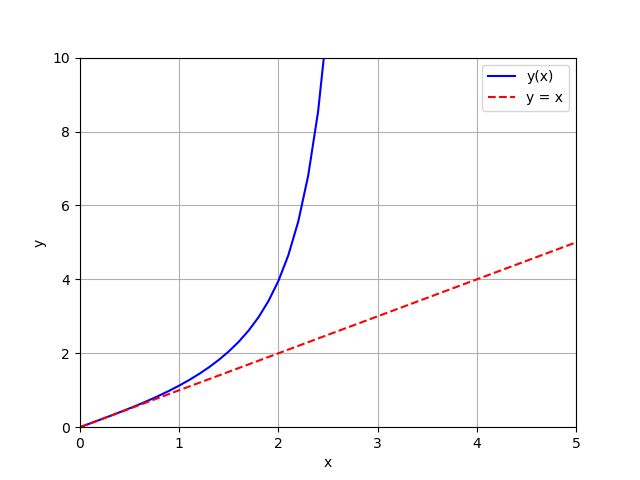
\includegraphics[width=1\textwidth]{figs/fig.png}
	\label{fig:Plot1}
\end{figure}



\end{document}
